\documentclass{article}
\usepackage{tikz}
\usepackage[compat=1.1.0]{tikz-feynhand}
\begin{document}
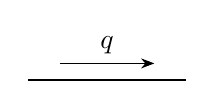
\begin{tikzpicture}
  \begin{feynhand}
    \vertex (a) at (0,0);
    \vertex (b) at (2,0);
    \propag[plain,mom={$q$}] (a) to (b);
  \end{feynhand}
\end{tikzpicture}

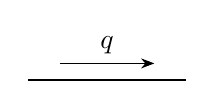
\begin{tikzpicture}
  \begin{feynhand}
    \vertex (a) at (0,0);
    \vertex (b) at (2,0);
    \propag[plain,momentum={$q$}] (a) to (b);
  \end{feynhand}
\end{tikzpicture}

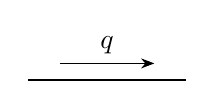
\begin{tikzpicture}
  \begin{feynhand}
    \vertex (a) at (0,0);
    \vertex (b) at (2,0);
    \propag[plain,/tikzfeynhand/mom={$q$}] (a) to (b);
  \end{feynhand}
\end{tikzpicture}

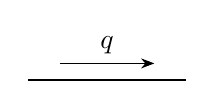
\begin{tikzpicture}
  \begin{feynhand}
    \vertex (a) at (0,0);
    \vertex (b) at (2,0);
    \propag[plain,/tikzfeynhand/momentum={$q$}] (a) to (b);
  \end{feynhand}
\end{tikzpicture}
\end{document}
